\section{数値的な図示と今後の問題}
\label{sec:numerical}

本節の図示は、参照球面の公式~\eqref{eq:reference_energy}から、
通常の浮動小数点演算を用いて直接再計算したものである。
これらは提案する分類の幾何を目に見える形にするものであり、
計算主張C1--C6への入力ではない。
付属のソース一式には、描画コード、標本値、
求積の次数、および図~\ref{fig:branches}で用いた
有理スライスの記録が含まれる。

\subsection{枝と子午線断面}

軸上では、回転対称性により方位角についての積分が
厳密に消える。正の根を69個のパラメータにおいて
768点のGauss--Legendre則で求め、384点の則と比較した。
計算された根の変化は最大で$9.87\times10^{-7}$であった。
扁長側の枝は、65個のパラメータにおいて
$192\times384$の極角–方位角則で計算した。すべての根は、
遷移パラメータから離れたところで、挟み込みとスカラーの求根法によって
得た。二つの求積解像度の間の食い違いは
診断であって、厳密な誤差評価ではない。

\begin{figure}[tbp]
\centering
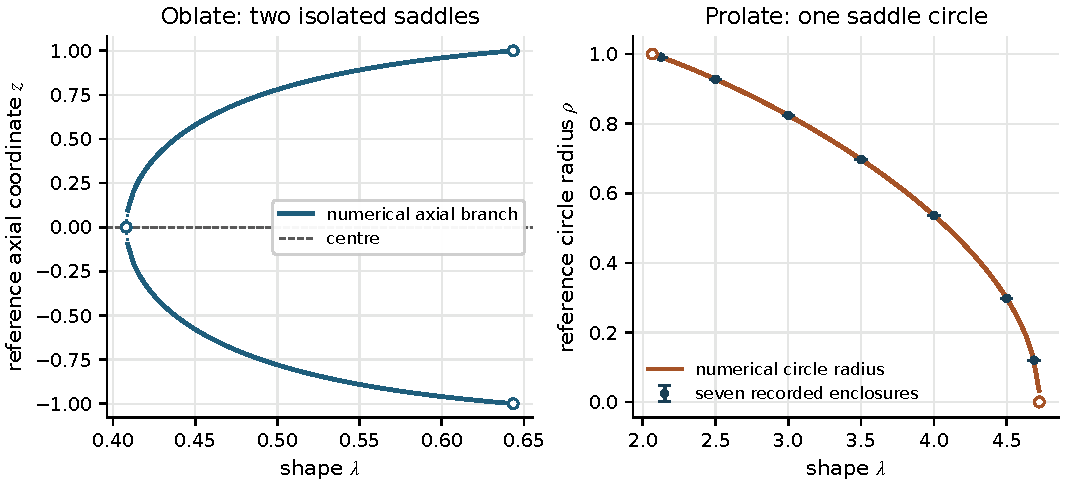
\includegraphics[width=\linewidth]{figures/branches.pdf}
\caption{参照座標において数値的に計算した、中心以外の
枝。左：扁平側の二つの軸上の鞍点。
右：扁長側のただ一つの停留円の半径。
右図に印を付けた七つの縦の区間は、
窓パッケージに記録された厳密な有理スライス包囲であり、その
幅はほとんどが描画の解像度より小さい。これらは
そのパッケージの証拠としての位置づけを引き継ぐ。白抜きの端点記号と点線の
接続は、分類された極限を示すものであり、追加の
数値的な根の計算を示すものではない。中心は全域で存続する。}
\label{fig:branches}
\end{figure}

図~\ref{fig:energy}のエネルギー断面では、
$128\times256$の球面則と$99\times99$の子午線格子を用い、
$q_1^2+q_3^2\leq0.98^2$を満たす7,525個の点を残した。
外縁の小さな部分を省いてあるので、有限解像度の画像が、
境界トレースが標本化によって確立されたかのように示唆することはない。
各パネルはそれぞれ固有のエネルギー尺度をもつ。扁長側の円の領域では、
子午線平面内の二つの十字は、一つの連結な
停留円との交点であり、二つの孤立した停留点ではない。

\begin{figure}[tbp]
\centering
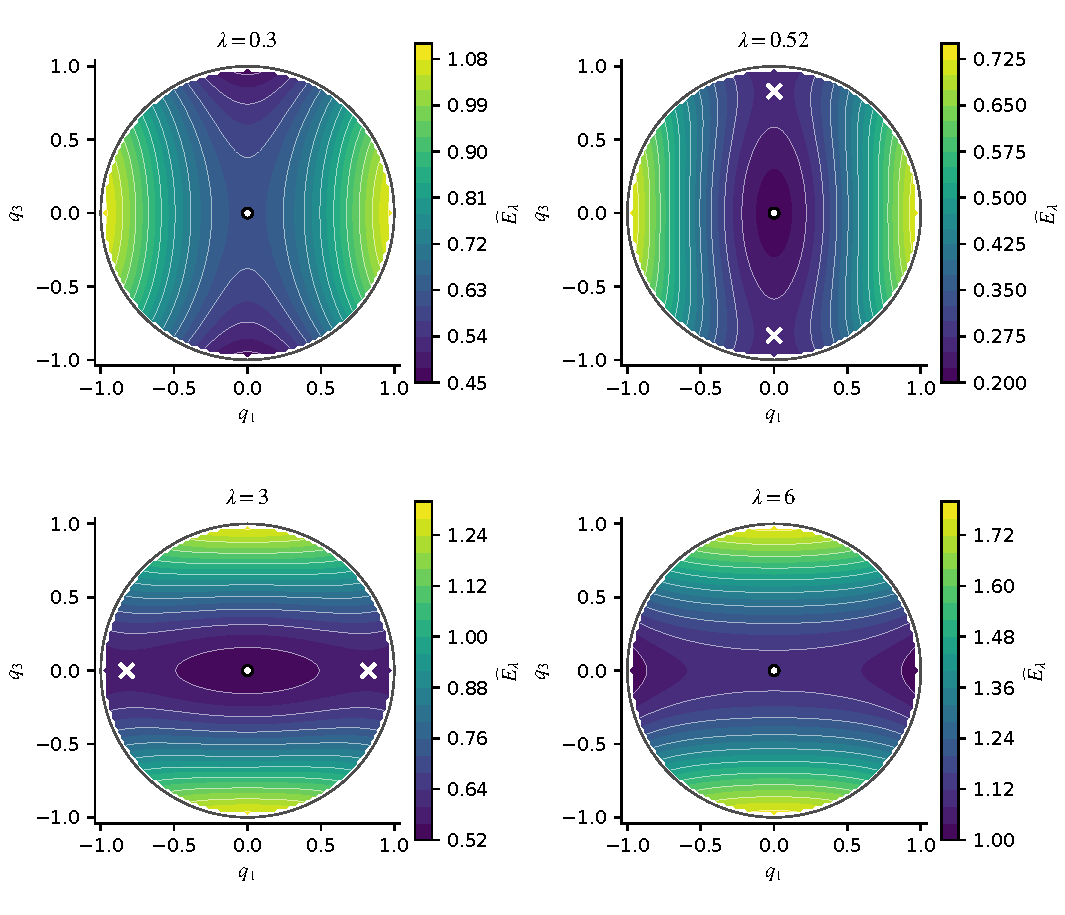
\includegraphics[width=.96\linewidth]{figures/energy_sections.pdf}
\caption{$\lambda=0.3,0.52,3,6$に対する$\widehat E_\lambda$の
参照座標での子午線断面。白い円板は中心を示し、白い十字は
中心以外の停留交点を示す。四つのパネルは
順に、中心の鞍点、中心の極小と
軸上の鞍点対、中心の極小と鞍点円、および
指数2の中心の鞍点を示す。各パネルの周りに描いた円は
参照境界であり、エネルギーは
半径$0.98$までしか標本化していない。これらは区間演算によらない数値的な図示である。}
\label{fig:energy}
\end{figure}

\subsection{記録された符号の余裕の大きさ}

定数$16189/2^{36}$と$3341881/2^{36}$は、
パラメータと空間の箱全体にわたる区間包囲から得られる、
小さな正の残余の余裕である。これらは
$V$の実際の大域的最小値の推定値ではなく、報告の単位$2^{-36}$は
包囲の誤差全体を測るものでもない。
繰り返し現れる変数の間の依存性、角度の値域の過大評価、および外側の箱の
幅は、いずれも符号の余裕の大部分を消費しうる
\citep{Rump2010}。C4の二つの縦方向の窓について、報告された$E_{zz}$と$E_z$の箱全体での余裕は、それぞれおよそ$1.75\times10^{-4}$と$4.86\times10^{-5}$である。別個の数値的な検討では、それぞれの窓で標本上の最小値が$1.07$と$0.32$の近くにあると報告された。この数桁の開きは包囲による損失を例示するものであり、標本上の最小値は連続体上の下界を与えない。尺度の比較として有用なのは、
$\rho=z=0.2$における直接の点値である：
\begin{center}
\begin{tabular}{rrr}
\toprule
$\lambda$&$V(0.2,0.2;\lambda)$&$H(0.2,0.2;\lambda)$\\
\midrule
1&1.261673&1.261673\\
1.5&1.810885&0.883353\\
2&2.053848&0.593574\\
3&2.169992&0.242475\\
5&2.025279&$-0.042247$\\
\bottomrule
\end{tabular}
\end{center}
求積則を$128\times256$から$256\times512$へ倍にしても、
これらの点値の変化は高々$1.65\times10^{-14}$である。
この一致は桁を認証するものではなく、
連続体上の下界を与えるものでもない。これは、記録された下端が非常に小さくても、
典型的な内点で導関数がほとんど消えていることを
必ずしも意味しない理由を例示するにすぎない。

\subsection{軸方向の凹性の拡張の可能性}

解析的な凹性の補題は、
$0<\lambda\leq1/32$に対する一様評価を証明する。符号に関する次のより強い言明が成り立てば、
残りの扁平側の解析の多くが簡単になる。

\begin{conjecture}\label{conj:concavity}
すべての$0<\lambda<\cO$と$|q|<1$に対して、
\[
 \partial_{zz}\widehat E_\lambda(q)<0.
\]
\end{conjecture}

$96\times192$の球面則による数値的な確認では、
$\lambda=1/16,1/8,1/4,0.35,0.4,0.4079$のそれぞれについて、
半径$0.96$の非負の子午線四分円板内の
473個の点を標本とした。
標本値はすべて負であった。これらの有限
標本における最大値は、それぞれおよそ
$-0.223524,-0.367927,-0.328099,-0.138342,-0.019734$、
および$-0.000147$であった。
さらに、境界に近い八つの弧のそれぞれの上で、等間隔な17個の子午線角において弦Hessianの求積を行ったところ、標本値はすべて狭義に負であった。$\lambda=1/128,1/64,1/32$に対しては半径$0.9999$を用いた。$\lambda=0.25,0.35,0.4,0.4079,0.42$に対しては$0.9995$を用いた。二つの組において、負の度合いが最も小さい標本値は、それぞれおよそ$-0.031$と$-0.487$であった。これらは点ごとの診断である。とくに、$0.42>\cO$は予想の範囲外にあり、そこでは中心がすでに正の軸方向曲率をもつ。

最大値がつねに中心でとられるという主張は
より強いものであり、すべての標本がそれを示唆しているわけではない：
$\lambda=1/8$では、$(\rho,z)=(0.88,0)$における値はおよそ
$-0.367927$であり、中心での値$-0.383316$より大きい。
$1/4$から$0.4079$までの四つの標本パラメータについては、
標本上の最大値は確かに中心でとられる。
予想~\ref{conj:concavity}は
最大値の位置についての主張を含まず、本節のいかなる計算も、
既存の証明義務を取り除くためには用いていない。

\subsection{三軸に関する具体的な問題}

$\lambda$を$(\bP,\cP)$の真に内側に固定し、
$M_\lambda$を次で置き換えて回転対称性を破る：
\[
 M_{\lambda,\epsilon}
 =\diag(e^\epsilon,e^{-\epsilon},1)M_\lambda.
\]
その行列式は1のままである。停留円の
分類を仮定すると、摂動前の円に沿う法方向のHessianは
可逆である。したがって陰関数定理により、
その円の近くで二つの法方向の臨界方程式が解かれ、
残りの方程式は周期的な角度エネルギー
$\Psi_\epsilon(\phi)$に帰着される。
第一変分は
$T=\diag(1,-1,0)$について線形である。このテンソルを$\phi$だけ回転すると、
角度の重み2の余弦成分と正弦成分が生じ、
$q_2=0$に関する鏡映により、$(\rho_*,0,0)$における正弦成分は
消える。法方向の補正の一次の寄与は、
摂動前の勾配が零であるため消える。
したがって、
$A(\lambda)=\left.\partial_\epsilon
\widehat E_{\lambda,\epsilon}(\rho_*,0,0)\right|_{\epsilon=0}$とおくと、
簡約された展開は
\[
 \Psi_\epsilon(\phi)
 =\Psi_0+\epsilon A(\lambda)\cos(2\phi)
   +O_{C^2(S^1)}(\epsilon^2),
\]
となる（ただし$A(\lambda)\ne0$とする）。
十分小さい零でない$\epsilon$に対して、主要項の角度微分の四つの単純
零点は存続し、近くの臨界点を
尽くす。一意的な法方向の解に引き継がれる座標鏡映により、
それらは正確に
$\phi=k\pi/2$に、すなわち向かい合う二組の主軸上の対に位置する。
それらの角度方向の曲率は符号が交互に変わる。法方向のHessianのSchur補行列は、
簡約された角度方向の曲率との合同なブロック分解を
与える。二つの法方向の
曲率は互いに逆の符号を保つので、それらの点のうち二つは
Morse指数1をもち、二つは指数2をもつ。

厳密な角度方程式もある。正定値行列$C=L^TL$に対してエネルギーを$F(C,q)$と書き、対称行列$G$を$D_CF[U]=\operatorname{tr}(GU)$によって定める。半軸$\ell_i$をもつ主軸枠において$T_{ij}=2\ell_i\ell_jG_{ij}$とおく。任意の回転$R$に対して、参照積分変数の変換により$F(RCR^T,Rq)=F(C,q)$が成り立つ。$(1,2)$平面内の回転について微分すると、次を得る：
\[
 q_1E_2-q_2E_1=(\ell_2/\ell_1-\ell_1/\ell_2)T_{12}.
\]
同様に、上に示した対角変形の微分から、第一軸上の摂動前の円の点において$A=T_{11}-T_{22}$が得られる。この厳密な恒等式は、零でない変形においても成り立つ。

$\cP$の近くの固定した形状に対して、第一軸上の形状微分は$\rho$について滑らかで偶である。その定数項は、二つの赤道軸の入れ替えにより消える。よって、円が縮むとき$A=O(\rho_*^2)$である。一様に評価すべき自然な量は$A/\rho_*^2$である。通常の求積によると、$\lambda=2.1,3,4,4.7$においてそれぞれ$0.6744,0.5744,0.4879,0.4399$となる。枝全体における正の一様下界は、ここでは未解決の評価として残る。序論で引用した局所的な三軸の研究は、扁長側の中心遷移の近傍に関するものである。これら四つの標本も、厳密な角度方程式それ自体も、三軸族全体にわたって他の臨界点を排除するものではない。

\section{入手先、再現性、および草稿の状況}
\label{sec:availability}

計算に関する参照文献は、
公開リポジトリ\texttt{cotaxxxx/bg-spheroid-family}および
\texttt{cotaxxxx/bg-oblate-spheroid}内の固定されたコミットとパスを特定する。
それ以前の背景資料は公開リポジトリ
\texttt{cotaxxxx/basepoint-geometry}にある。扁平の極限の解析的な
議論と、扁長側の裾の議論のうち軸上の部分は、
固定された研究記録をもとに、ここで詳しく展開したものである
\citep{data-oblate-analytic,data-prolate-axis}。
球の場合の証明は第~\ref{sec:sphere}節で与えており、
未公表の球に関する原稿を必要としない。
記録V24（2026年11月16日）：\texttt{cotaxxxx/bg-spheroid-family}、
コミット\texttt{127be52046e9498d1306fe3d35c3e02e91c636de}、
ファイル\href{https://github.com/cotaxxxx/bg-spheroid-family/blob/127be52046e9498d1306fe3d35c3e02e91c636de/runs/2026-11-16/D_OB_GLOBAL_CLOSED_V24/JUDGE_RULING_D_OB_GLOBAL_CLOSED_20261116.md}{\path{JUDGE_RULING_D_OB_GLOBAL_CLOSED_20261116.md}}%
（日本語の作業記録）。この一次記録の正確な写しは、
付属のソース一式の\path{provenance/V24/}以下に含まれている。
付属のプロジェクト水準のAI監査は、組み立ての議論と
出典の参照を点検した。選ばれた区間箱の計算は
独立に再計算され、厳密な整数被覆検査が
\path{CURRENT_REPRODUCTION_v0_5_4.md}に記録された範囲で行われたが、
この監査もそれらの検査も、C1--C6の完全な再実行には当たらない。

主張ごとの再現の対応表については、ソース一式内の
\path{CURRENT_REPRODUCTION_v0_5_4.md}を見よ。これは、
C1--C6を、固定された入力パッケージ、生成および検査のコマンド、
台帳のパス、独立な再評価の範囲とともに、
残してある過去の\path{REPRODUCTION.md}とは別に列挙する。この新しい対応表は、
列挙された元の生成プログラムがすべて再実行されたとも、
その元の解析的な核が独立に再導出されたとも主張しない。

付属の改訂版一式には、原稿のソース、
文献データ、ベクター形式の図、図のデータと再現用スクリプト、
および固定された計算ソースの対応表が含まれる。これは、
すべての上流の計算についての完全な認証済みアーカイブではない。
そのような統合された証明パッケージに対するアーカイブ用DOIは、
この改訂版では主張しない。固定されたリリースには、厳密な
入力の箱、選ばれたすべての最終の葉、係数表、
生成プログラムと検査プログラムのソース、ビルド環境、実行
コマンド、およびファイルのハッシュを、C1--C6から
対応する受理済みの記録への直接の対応表とともに含めるべきである。

互いに異なる三つの義務、すなわち解析的な
核の正しさ、その実装における正しい外向き演算と誤差上界、
および分類で用いる領域被覆の
完全性がある。ファイルのハッシュが確立するのは同一性であって、
これらの数学的性質のいずれでもない。元の
核による再現と、別途導出した核による再評価とは、
異なる失敗の様式に対処する。完全に独立な数値的再実行は
ここでは主張せず、その現在の範囲は
第~\ref{subsec:computational-workload}節に述べてある。
補足資料は、再実行のコマンド、固定された所在、および選択規則を与える。ソース一式には、独立な区間計算とそれらの整数被覆検査が含まれる。

\paragraph{AIツールの使用。}
ChatGPT（OpenAI）は、探索的な導出、数値計算
コードと検証スクリプト、英語の文言の提案、
改稿、および組版を補助した。Codex（OpenAI）はコーディングと
原稿の検討を補助し、GPT-6.2 Astra（OpenAI）は研究設計と
専門的な計算作業を補助した。Claude（Anthropic）は、
議論の組み立て、出典の参照、および原稿の差分について、別個のプロジェクト水準のAI監査を
行い、Claude Code（Anthropic）は、記録された範囲で特別なコード
監査と独立な検査を提供した。Muse（Meta）は、
扁平側のD5の作業の一部を含む、選ばれた計算
資料について、追加の外部AI監査を行った。これらの記録は、
C1--C6の独立に実装された完全な再実行でも、外部の
人間による査読でもない。英語の初稿の段落と、
その後の翻訳または校正とを区別する来歴は、まだ完全には
再構成されておらず、したがって、「校正」に限定した説明は
主張しない。ソース一式にはAI来歴の検討記録が含まれる。
投稿先候補の学術誌の初稿に関する制限への適合は
主張しない。提案されたすべての主張、
文献、コードの寄与、および最終的な開示についての著者による検証は未了である。
